\phantomsection
\begin{appendices}
\titleformat{\section}
{\color{chambray}\normalfont\Large\bfseries}{}{1em}{}
\section{ANNEXES}
\markboth{ANNEXES}{}
\subsection{Présentation des principales interfaces d'Arkevia}
\null\vfill
\begin{figure}[H]
    \begin{center}
        
\includegraphics[width=\linewidth]{images/annexes/scr1.png}
        \caption{Page d'authentification Arkevia}
        \label{fig:arkevia1}
    \end{center}
\end{figure}
\vfill\null
\clearpage
\null\vfill
\begin{figure}[H]
    \begin{center}
        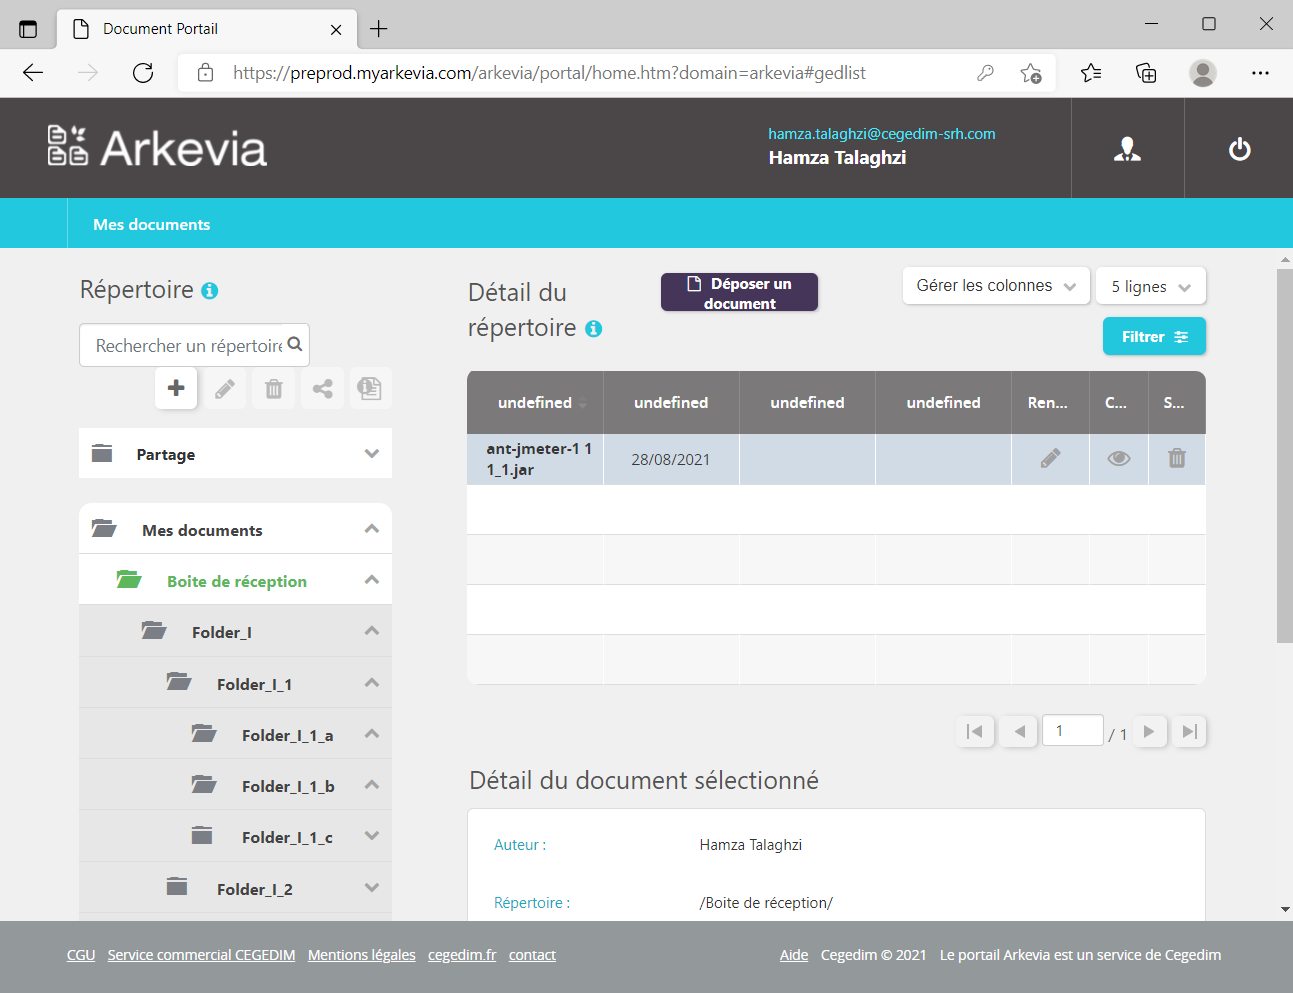
\includegraphics[width=\linewidth]{images/annexes/scr2.png}
        \caption{Page de gestion des documents}
        \label{fig:batch}
    \end{center}
\end{figure}
\vfill\null
\begin{figure}[H]
    \begin{center}
        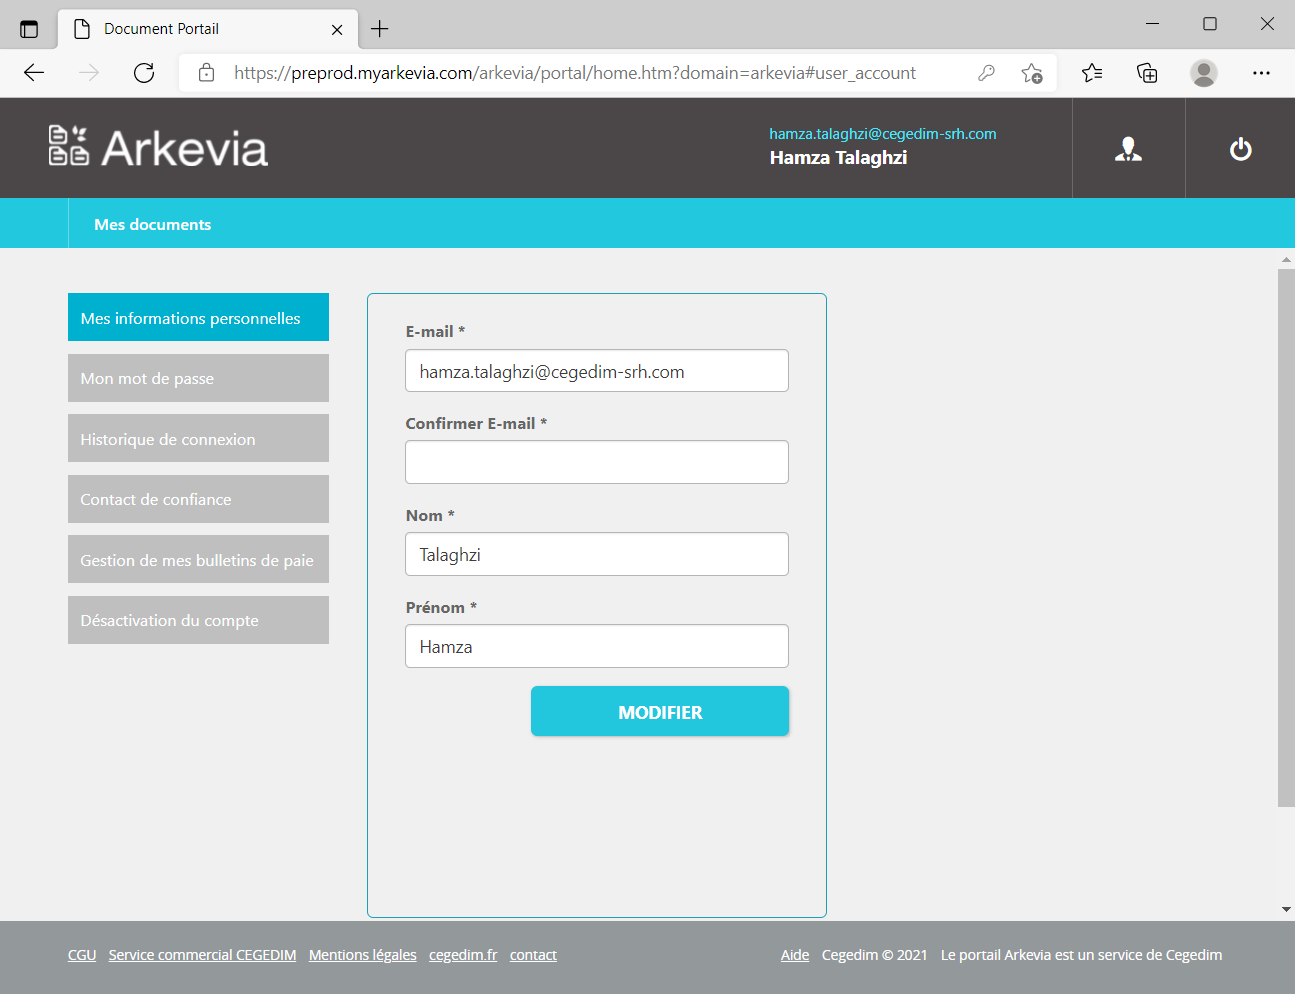
\includegraphics[width=\linewidth]{images/annexes/scr3.png}
        \caption{Page de gestion de compte Arkevia}
        \label{fig:batch}
    \end{center}
\end{figure}
\subsection{Audit de code : checklist élaborée par Cegedim SRH}
\label{sec:checklist}
\begin{longtblr}[caption={Extrait des règles et pratiques de développement logiciel instaurées par Cegedim SRH}, label={tab:dev}]{
    hlines = {0.25pt,azure6},
    vlines = {0.25pt,azure6},
    colsep=4pt,
    rowsep=4pt,
	colspec={QX},
}
\textbf{Réf.} & \textbf{Description de la règle}\\
RG\_DEV\_GN\_001 & Single responsibility principle :
Une fonction doit être responsable d'une et d'une seule tâche. Lorsqu'une fonction fait plus d'une tâche, elle est plus difficile à composer, à tester et à comprendre.\\
RG\_DEV\_GN\_002 & Don't repeat yourself :
Souvent, nous avons du code en double parce que nous avons deux ou plusieurs choses légèrement différentes, qui partagent beaucoup en commun, mais leurs différences nous obligent à avoir deux ou plusieurs fonctions distinctes qui font en grande partie les mêmes choses. Supprimer le code en double signifie créer une abstraction qui peut gérer cet ensemble de choses différentes avec une seule fonction / module / classe.
Factoriser le code en double.\\
RG\_DEV\_GN\_003 & Open/Closed principle :
Les nouvelles fonctionnalités ne doivent pas modifier le code existant.\\
RG\_DEV\_GN\_004 & Test unitaire :
Chaque fonction doit être testée avec au minimum un cas passant et un cas non passant.\\
RG\_DEV\_GN\_005 & Respect des warnings eslint sonarLint :
Veiller au maximum à ce qu’il n’y a pas de warnings eslint et/ou sonarlint dans la classes/ou parties de classes impactées dans le cadre d’une évolution, l’objectif est d’atteindre 0 Warnings dans le possible.\\			
RG\_DEV\_GN\_006 & Correction des NullPointerException :
Éviter de contourner le problème de nullité en ajoutant des tests, et aller plus en profondeur dans le diagnostic pour détecter l’origine du problème et le résoudre d’une manière radicale.\\
RG\_DEV\_GN\_007 & Arguments de fonctions :
Limiter le nombre de paramètres d'une fonction est extrêmement important, un ou deux arguments est le cas idéal, et trois devraient être évités si possible. Rien de plus que cela devrait être utilisé. Utiliser des objets si nous avons besoin de beaucoup d'arguments.\\			
RG\_DEV\_GN\_008 & Cas des dépassements de capacité :
Éviter de contourner le problème en tronquant des valeurs, et aller plus en profondeur dans le diagnostic pour détecter l’origine du problème et le résoudre d’une manière radicale.
% RG_DEV_GN_008	O		Cas des « prepared statement »  :
% Utiliser systématiquement les « prepared statment » à chaque fois quand c’est possible, et respecter la charte de nommage sur la partie PS.			
% RG_DEV_GN_009	O		Code en dur dans les programmes 
% Eviter le code en dur dans les programmes pour une meilleure évolutivité			
% RG_DEV_GN_010	O		Table en mémoire :
% Eviter de charger les tables en mémoire pour de meilleures performances.
% Exemple :
% Ne pas charger toutes les données d'une table de référence dans une liste d'objets.			
% RG_DEV_GN_011	O		Valeurs par défaut :
% Privilégier l'utilisation des valeurs par défaut dans les fonctions.			
% RG_DEV_GN_012	O		Eviter l'utilisation des flags comme des paramètres de fonction
% Diviser les fonctions si elles suivent des chemins de code différents en fonction d'un booléen.			
% RG_DEV_GN_013	O		Eviter les conditions négatives			
% RG_DEV_GN_014	O		Eviter les conditions imbriquées (au dessous 2 niveaux )			
% RG_DEV_GN_015	O		Supprimer le code mort			
% RG_DEV_GN_015	O		Privilégier l'utilisation des getters et des setters			
% RG_DEV_GN_016	O		Nomenclature :
% Utiliser des noms de variables, de fonctions et de classes significatifs et pronoçables:			
% RG_DEV_GN_017	O		• Un identifiant représentant une collection d’objets doit être un nom au pluriel (utiliser de préférence le nom de l’objet) précédé de "list".
% Exemple :
% private String[] listCountries = null;
% private Personne[] listPersonnes = null;			
% RG_DEV_GN_018	O		• Le terme compute doit être employé dans les méthodes où quelque chose est calculé. Il donne au lecteur l'indice immédiat que c'est potentiellement une opération longue.			
% RG_DEV_GN_019	O		• Le terme find doit être employé dans les méthodes où quelque chose est recherché. Elle donne au lecteur l'indice immédiat que la méthode est une simple recherche avec un minimum de calculs.
% Exemple :
% matrice.findMinElement()			
% RG_DEV_GN_020	O		• Le terme initialize doit être employé là où un objet ou un concept est construit. L'abréviation d'init peut également être employée.
% Exemple :
% printer.initializeFontSet();
% printer.initFontSet();			
% RG_DEV_GN_021	O		• Des noms de concept complémentaire doivent être employés pour des comportements complémentaires.
%  get/set, add/remove, start/stop, insert/delete, increment/decrement, old/new, begin/end, first/last, up/down, min/max, next/previous, old/new, open/close, show/hide, create(ou New)/destroy.			
% RG_DEV_GN_022	O		• Les méthodes de mise à jour, suppression et insertion de données sont préfixées respectivement par update, delete et insert.			
% RG_DEV_GN_023	O		• Les constantes d'un même concept doivent être réunies et préfixées par un nom commun de type. Ceci indique que les constantes appartiennent au même ensemble, et permet d'identifier le concept représenté.
% • Attention néanmoins à éviter les tautologies (par exemple : Color.COLOR_RED).
% Exemple :
% static final int COLOR_RED   = 1;
% static final int COLOR_GREEN = 2;
% static final int COLOR_BLUE  = 3;			
% RG_DEV_GN_024	O		Commit tout azimut :
% Eviter de mettre des Commit/Rollback intermédiaires dans les étapes des étapes du Batch, un commit ou Rollback doivent être positionnés à la fin des étapes. 			
% RG_DEV_GN_025	O		Commentaire :
% Mettre un nombre de commentaires considérable pour décrire ce que font les modifications ajoutées, avec un contenu explicite, clair et compréhensible sur ce que fait réellement le code.
% Utiliser au max les formats conventionnés (JSDOC, JavaDoc, ,,,) pour les commentaires			
% Charte Java						
% RG_DEV_JAVA_001	O		Nom Package :
% • Le préfixe d'un nom de package doit correspondre au niveau supérieur d'un nom de domaine : com
% Exemple : 
% package com.ro.framework.batch;			
% RG_DEV_JAVA_002	O		Décomposition domaine : 
% • Un domaine est décomposé en plusieurs procédures.
% Exemple : 
% package com.ro.domaine.procedure;			
% RG_DEV_JAVA_003	O		Nom Classe :
% • Le nom d'une classe ne doit pas comporter d'information concernant son mode d'implémentation, celui-ci pouvant évoluer pendant le cycle de vie de l'application.			
% RG_DEV_JAVA_004	O		• Si le nom d'une classe comporte des informations concernant son type technique (Exception, Trace, Objet métier, etc.) ou le type de concept implémenté (Factory, Facade, etc.), ces informations doivent être suffixées.
% Exemple :
% class IRuntimeNavigationFactory // Interface d’une fabrique/usine
% class NavigationFactoryBuilder  // Fabrique d’usine
% class BeneficiaireSingleton  // Singleton
% class ProcessAccessCfg // Configuration
% class TechnicalException // Exception technique
% class DevisBOModel  // Modèle métier
% class MethodInvokerTools // Utilitaires
% class ProcessAccessManagerTest // Test			
% RG_DEV_JAVA_005	O		• Il est courant de créer une implémentation simpliste de classe ou d'une interface fournissant le comportement par défaut aux méthodes d'interface. Dans ce cas, l'implémentation peut être suffixée par Default.
% Exemple :
% class DefaultManager implements IManager;			
% RG_DEV_JAVA_006	O		• Une normalisation particulière est appliquée aux classes Actions.
% • Mot Clé « Map » suivi d’un mnémonique pour le mapping.
% • Mot Clé « Pop » suivi d’un mnémonique pour le populing.
% Exemple :
% class MapListePersonnes;
% class PopListePersonnes;			
% Charte JavaScript						
% RG_DEV_JS_001	O		Déclaration des variables:
%     * Utiliser "const" par défaut
%     * Utiliser "let" si la variable va être modifier
%     * Ne pas utiliser "var"			
% RG_DEV_JS_002	O		Modifier un objet ou un tableau au sein d'une fonction risque d'avoir des effets secondaires.
% La solution est de cloner le tableau / objet par la fonction, modifier et ensuite renvoyer la clone, ça garantit que les autres fonctions qui utilisent toujours l'ancien tableau / objet ne seraient pas affectées par les modifications.			
% RG_DEV_JS_003	O		Tyepes des variables :
% Etant donné que JavaScript n'est pas langage typé, éviter au maximum la vérification du type:
%     * instanceof
%     * typeof			
% RG_DEV_JS_004	O		Traitements asynchrones :
% Privilégier l'utilisation des "promises" au lieu des "deffered"
% Ne pas ignorer les promesses rejetées			
% Charte VueJS						
% RG_DEV_VUE_001	O		• Tous les noms de composants doivent être en minuscule,
% Exemple : register-component.vue			
% RG_DEV_VUE_002	O		Les noms de composant devraient toujours être des mots multiples (separés par un tiret), à l’exception du composant racine App et des composants préconçus fournis par Vue comme <transition> ou <component>. (pour prévenir les conflits)
% Exemple:
% register-header-component.vue			
% Charte MongoDB						
% RG_DEV_MONGO_001	O		La taille maximale d'un document MongoDB est de 16MB			
% RG_DEV_MONGO_002	O		Nom Collection et Index :
% - Noms en minuscules: évite les problèmes de sensibilité, les noms de collections MongoDB sont sensibles à la casse.
% Pluriel: plus évident pour étiqueter une collection de quelque chose comme pluriel, par exemple “fichiers” plutôt que “fichier”

% - Pas de séparateur de mots: évite les problèmes où des personnes différentes (à tort) séparent les mots (username <-> user_name, first_name <-> firstname). .

% - Notation par points pour les collections plus détaillées: donne des indications sur la manière dont les collections sont liées. Par exemple, vous pouvez être raisonnablement sûr de pouvoir supprimer “users.pagevisits” si vous avez supprimé “users”, à condition que les personnes qui ont conçu le schéma aient fait du bon travail.			
% RG_DEV_MONGO_003	O		Nom Collection et Index :
% - Noms en minuscules: évite les problèmes de sensibilité, les noms de collections MongoDB sont sensibles à la casse.
% Pluriel: plus évident pour étiqueter une collection de quelque chose comme pluriel, par exemple “fichiers” plutôt que “fichier”

% - Pas de séparateur de mots: évite les problèmes où des personnes différentes (à tort) séparent les mots (username <-> user_name, first_name <-> firstname). .

% - Notation par points pour les collections plus détaillées: donne des indications sur la manière dont les collections sont liées. Par exemple, vous pouvez être raisonnablement sûr de pouvoir supprimer “users.pagevisits” si vous avez supprimé “users”, à condition que les personnes qui ont conçu le schéma aient fait du bon travail.			
% RG_DEV_MONGO_004	O		Plutôt que de récupérer l'intégralité du document, de mettre à jour les champs, puis de réenregistrer le document dans la base de données, émettez plutôt une mise à jour sur des champs spécifiques. Cela présente l'avantage de réduire l'utilisation du réseau et la surcharge de base de données.			
% Charte de structure et organisation						
% RG_STRUCT_001	O		Conventions de nommage :
%     * Les noms des composants de la libSmart: cs-xxx-yyy
%     * Les noms des fichiers des composants vue: csXxxYyy
%     * Les noms des composants métiers: camelCase
%     * Les noms des fichiers JS des composants métiers: camelCase
%     * Les noms des variables: camelCase
%     * Les noms des classes CSS: cs-xxx-xxx
%     * Les noms des scripts: wc_xxxYyy
%     * Les noms des libelles: snacke_case
%     * Les noms des méthodes: camelCase			SMART
% RG_STRUCT_002	O		Architecture du projet :
%     * Chaque module doit avoir son propre dossier
%     * Chaque module doit avoir son propre fichier de style
%     * Chaque module doit avoir son propre store
%     * Le composant métier doit être découpé:
%         ** Un fichier JS pour son template
%         ** Un fichier JS pour son script			SMART
% RG_STRUCT_003	O		Chemin d'accès :
% • Les pages sont situés sous " <APP> \sy-portal\HS-SY-Portal\src\main\webapp\portal\client"
% Exemple : <APP> \sy-portal\HS-SY-Portal\src\main\webapp\portal\client\arkevia\home\home-component.vue			ARKEVIA
% RG_STRUCT_004	O		Architecture du projet:
%     * Chaque composant doit appartenir à un seul module 
%     * Chaque composant doit inclure son propre fichier ts (logique du composant) et son fichier de vue (html)
%     * Un composant peut inclure son propre fichier de style 
%     * Un composant peut utiliser d'autres fichiers de style			MOBILE

\end{longtblr}
\subsection{Outils utilisés pour la réalisation de ce rapport}
Ce rapport est basé sur un modèle de rapport pédagogique conçu pour le département d'informatique de l'Université d'Avignon, par son auteur Vincent Labatut.\\
Pour obtenir ce modèle, veuillez visiter le site suivant : \url{https://fr.overleaf.com/latex/templates/modele-de-rapport-avignon-universite/pdbgdpzsgwrt}.\\

Le rapport est compilé à l'aide de \textbf{LuaLaTeX}, une variante de \textbf{LaTeX} utilisant le langage de script \textbf{Lua}. \textbf{LuaTeX} a été choisi comme successeur de \textbf{pdfTeX}. La structure générale et la plupart des commandes sont similaires à celles de LaTeX.\\

Il a également été utile d'utiliser certains supports pour produire les ressources et les illustrations incluses dans le rapport. Le tableau suivant rassemble les différents outils utilisés dans la mise en œuvre de ce rapport.
\begin{longtblr}[caption={Supports utilisés pour la réalisation de ce rapport}]{
    hlines = {0.25pt,cyan6},
    vlines = {0.25pt,cyan6},
    colsep=4pt,
    rowsep=4pt,
	colspec={cX},
    rowspec={Q[m] Q[m] Q[m] Q[m] Q[m] Q[m]},
}

{
\includegraphics[height=8mm]{images/annexes/adobecc.pdf}
 \\\textbf{Adobe Illustrator}
}
&  
Adobe Illustrator est un logiciel de création graphique vectorielle. Il fait partie de la gamme Adobe, peut être utilisé indépendamment ou en complément de Photoshop, et offre des outils de dessin vectoriel puissants. Les images vectorielles sont constituées de courbes générées par des formules mathématiques.\\
{
\includegraphics[height=8mm]{images/annexes/draw.pdf}
 \\\textbf{Draw.io}
 }
 & 
 Draw.io est une application de création de diagrammes et schémas sous licence Apache disponible sous Windows, macOS, Linux, sous forme d’application web et intégrée à des services cloud tels Nextcloud ou Google Drive.
 \\
 {
\includegraphics[height=8mm]{images/annexes/figma.pdf}
 \\\textbf{Figma}
 }
 & Figma est un outil collaboratif de conception et de prototypage d'interfaces.\\
{
\includegraphics[width=8mm]{images/annexes/vscode.pdf} \\
\textbf{Visual Studio Code}
} & Visual Studio Code est un éditeur de code source puissant, développé par Microsoft. Il est disponible pour Windows, Mac et Linux.\\
\end{longtblr}
\end{appendices}